% !TeX root = ../main.tex
% ====================
% I. GIOI THIEU
% ====================
\section{Giới thiệu}

\subsection{Bối cảnh bài toán}
Cùng với sự phát triển của các hệ thống giám sát thông minh, bài toán nhận dạng
con người qua nhiều camera ngày càng nhận được nhiều sự quan tâm trong lĩnh vực
thị giác máy tính. Trong các môi trường như sân bay, nhà ga, trung tâm thương
mại hay khu vực công cộng, một người có thể xuất hiện ở nhiều camera khác nhau
với các điều kiện quan sát không đồng nhất. Do đó, việc xác định các hình ảnh
thu được từ nhiều camera có thuộc cùng một người hay không là một bài toán có ý
nghĩa thực tiễn cao.

Bài toán này là \textbf{Person Re-identification (Person ReID)}. Mục tiêu của
Person ReID là tìm kiếm hoặc xác định lại một người trong tập ảnh hoặc video
được thu thập từ nhiều camera khác nhau. Đây là một hướng nghiên cứu quan
trọng, có nhiều ứng dụng trong giám sát an ninh, phân tích hành vi và quản lý
di chuyển trong không gian công cộng.

\begin{figure}[!htbp]
    \centering
    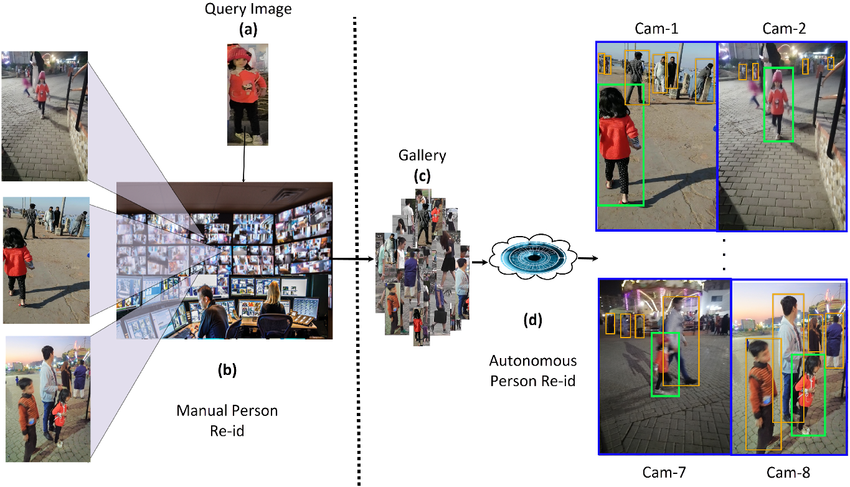
\includegraphics[width=\linewidth]{figures/smart-person-re-identification.png}
    \caption{Minh họa bài toán Person Re-identification trong hệ thống giám sát nhiều camera.}
    \label{fig:reid_example}
\end{figure}

Tuy nhiên, Person ReID là một bài toán khó do sự thay đổi lớn về
góc nhìn, ánh sáng, tư thế, độ phân giải ảnh và hiện tượng che khuất giữa các
camera. Cạnh đó, sự tương đồng về trang phục hoặc ngoại hình giữa nhiều
người khác nhau cũng làm gia tăng khả năng nhầm lẫn.

\subsection{Vấn đề nghiên cứu}
Trong những năm gần đây, các phương pháp học sâu đã cho thấy hiệu quả nổi bật
trong bài toán Person ReID nhờ khả năng học đặc trưng trực tiếp từ
dữ liệu. Nhưng hiệu quả của mô hình vẫn chịu ảnh hưởng bởi sự đa dạng của dữ
liệu, khả năng biểu diễn đặc trưng và cách đo lường độ tương đồng giữa các đối
tượng.

\begin{figure}[t]
    \centering
    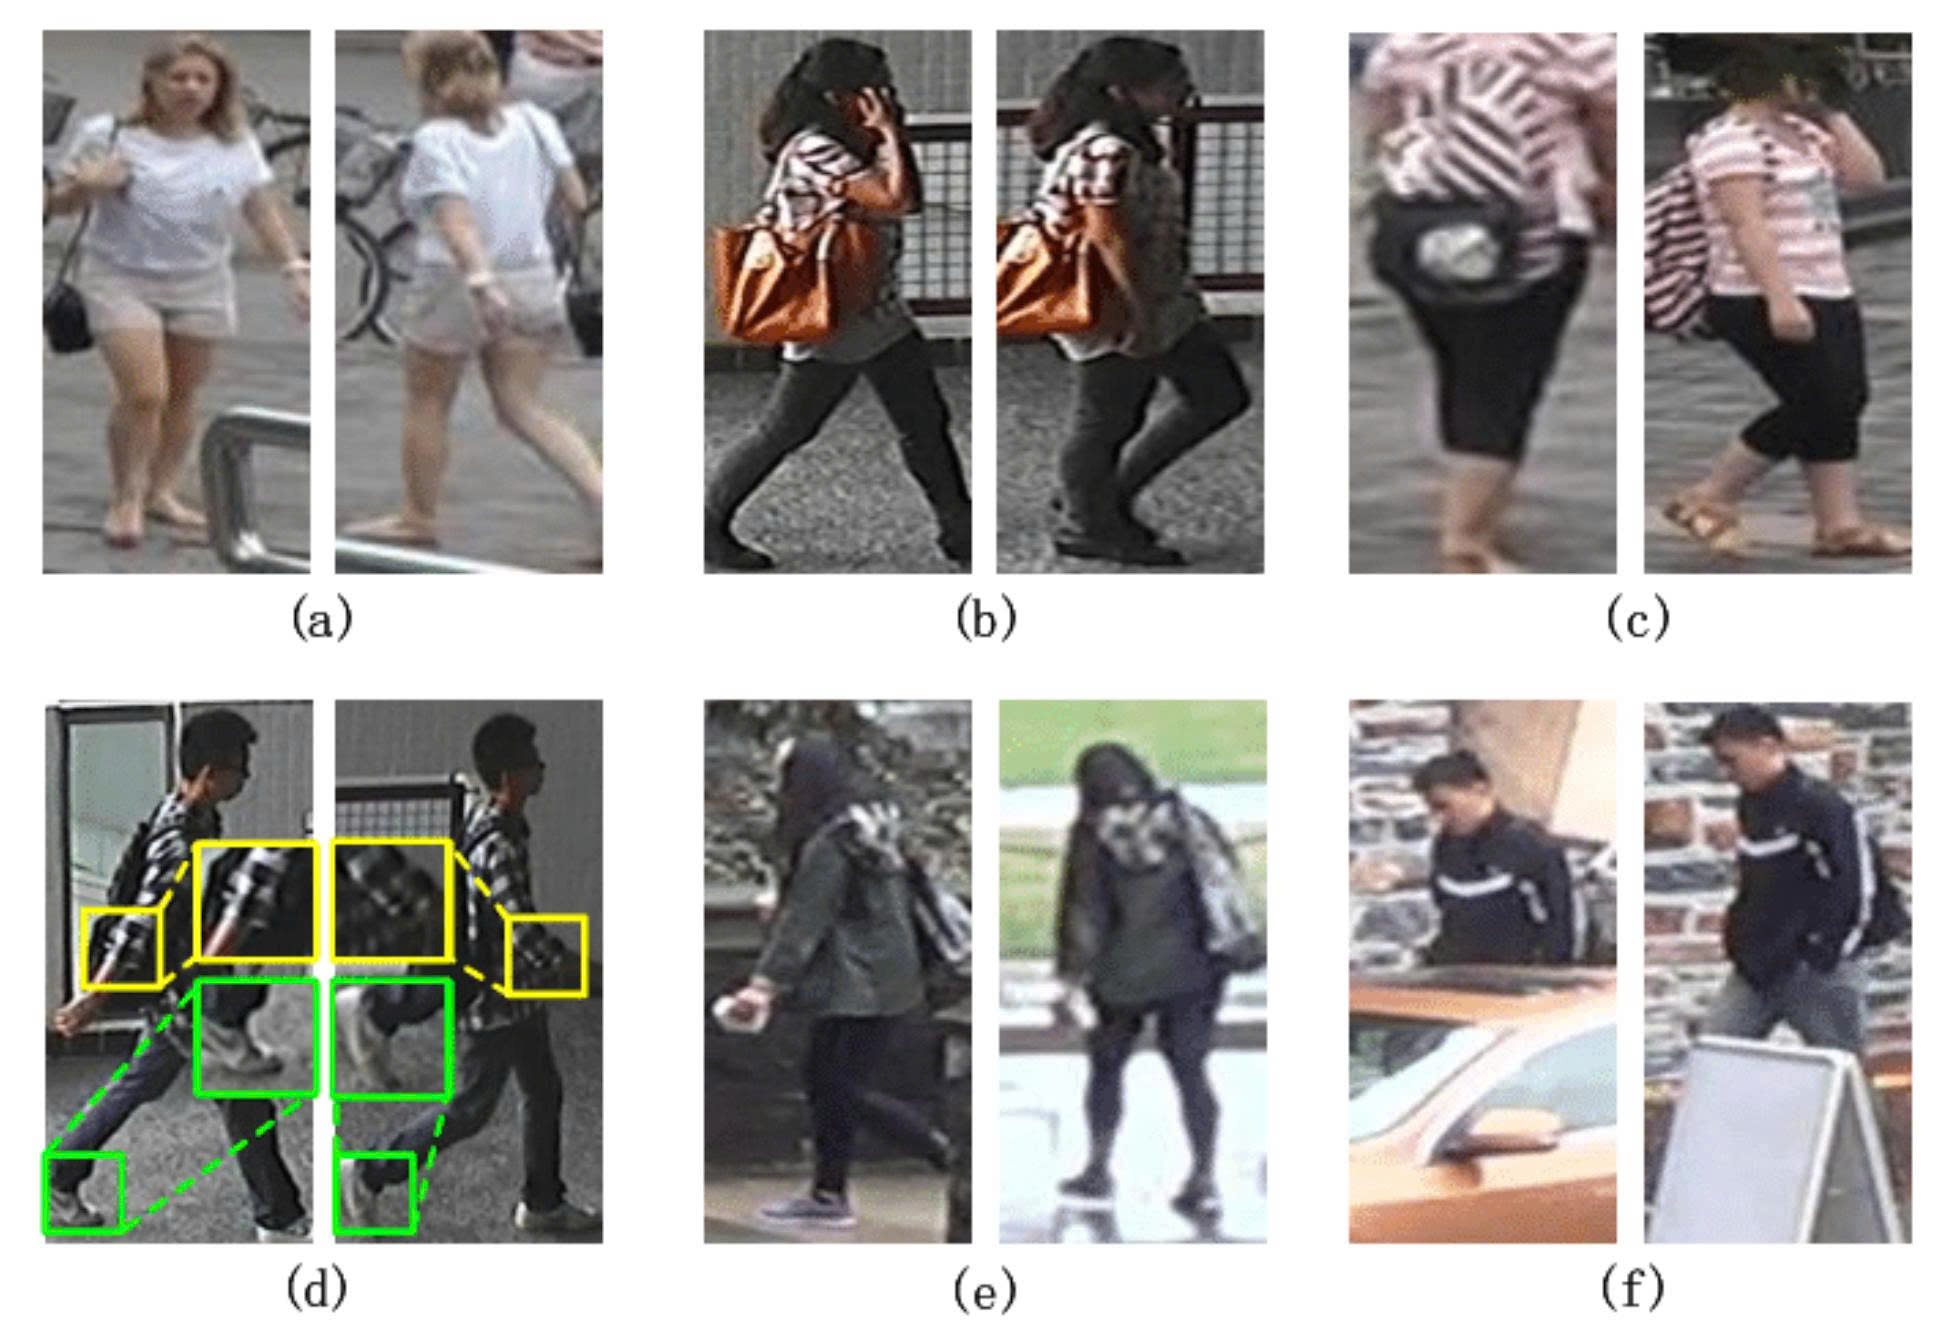
\includegraphics[width=0.9\linewidth]{figures/person-re-identification-challenges.jpg}
    \caption{Một số thách thức chính trong bài toán Person Re-identification, bao gồm thay đổi góc nhìn, tư thế, che khuất và nền nhiễu.}
    \label{fig:reid_challenges}
\end{figure}

Từ đó, đề tài đặt ra các vấn đề chính cần xem xét: các hướng tiếp cận hiện có
giải quyết bài toán, mô hình phù hợp để áp dụng trong phạm
vi đồ án, và những cải tiến giúp nâng cao hiệu quả nhận dạng khi
thực nghiệm trên tập dữ liệu chuẩn.
